\chapter{Capitolo 1: Concetti base di biologia}
La bioinformatica è una materia che tratta tanto l'informatica quanto la biologia, pertanto è necessario illustrarne gli argomenti più importanti, che verranno spiegati in modo funzionale allo scopo della presente tesi.
\newline
La \textit{biologia} è la scienza che studia la vita, dagli attori che ne fanno parte fino ai processi in cui essi sono coinvolti \cite{campbellBiology}. Poiché la vita sulla terra si estende dalle profondità del mare fino alla biosfera, si è reso necessario organizzarla in differenti ordini di grandezza. Tra le varie forme di vita si trovano,  in ordine crescente di dimensione ed omettendo quelle non interessate, le molecole (insiemi di atomi), le macromolecole (insiemi di molecole) e le cellule (insiemi di macromolecole).
\newline
Ci sono quattro tipi di macromolecole che sono essenziali per tutte le forme di vita:
\begin{itemize}
	\item \textit{Polisaccaridi}: macromolecole formate da aggregazioni di monosaccaridi, tra cui il fruttosio, il glucosio e così via. Sono riserve di energia pronta.
	\item \textit{Proteine}: sono la "struttura" degli esseri viventi, consentendo lo sviluppo e mantenimento degli organi.
	\item \textit{Lipidi}: chiamati anche grassi, sono le riserve energetiche di deposito.
	\item \textit{Acidi nucleici}: DNA e RNA, contengono e trasportano l'informazione genetica.
\end{itemize}
Di seguito vengono approfonditi il DNA, l'RNA e le proteine.
\newpage

\section{DNA}
Il \textit{DNA} o \textit{acido desossiribonucleico} è una macromolecola contenente il patrimonio genetico\footnote{Il patrimonio genetico contiene tutte le informazioni genetiche di un organismo.} degli esseri viventi \cite{campbellBiology}, pertanto ne detiene l'informazione ereditaria \cite{BiologySolomon}, che prende il nome di \textit{gene}.
\newline
Di seguito viene illustrata un'immagine del DNA, insieme ad una breve descrizione.
\newline
\begin{figure}[h!]
	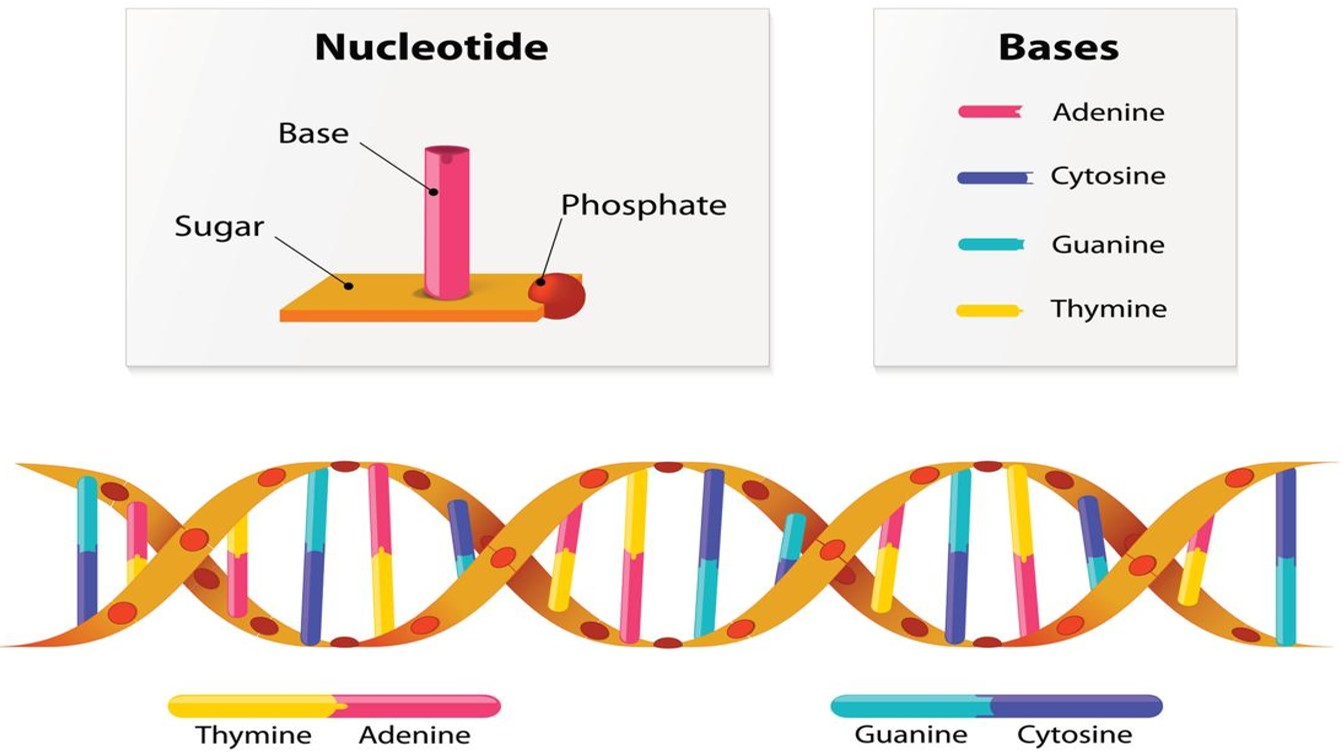
\includegraphics[width=\linewidth]{DNAStructure.jpg}
 	\caption{La struttura del DNA e del nucleotide.}
  	\label{fig:DnaAndNucleotideStructure}
\end{figure}
\newline
La struttura è caratterizzata da una doppia elica, dove ciascun filamento è formato da una sequenza di molecole di lunghezza variabile chiamate \textit{desossiribonucleotidi}.
\newline
Un desossiribonucleotide è composto da una molecola di zucchero, un gruppo fosfato ed una base azotata. Di quest'ultima, ne esistono quattro tipi:
\begin{itemize}
	\item \textit{adenina} (A);
	\item \textit{timina} (T);
	\item \textit{guanina} (G);
	\item \textit{citosina} (C).
\end{itemize}
Una proprietà importante delle basi azotate è che sono biunivocamente legate tra loro: l'Adenina si può legare solo con la Timina (A-T), mentre la Guanina con la Citosina (G-C). Questo significa che i filamenti sono complementari e quindi se conosciamo la sequenza di basi di un filamento di DNA sappiamo anche la sequenza di quello complementare.

\section{RNA}
L'\textit{RNA}, ovvero \textit{acido ribonucleico}, è una macromolecola caratterizzata da una struttura a singolo filamento composta da una \textit{sequenza di ribonucleotidi} di lunghezza variabile.
\newline
I ribonucleotidi si differenziano rispetto ai desossiribonucleotidi per una diversa molecola di zucchero e per la Timina (T) che è sostituita con l'Uracile (U).
\newline
Un tipo di RNA importante per la sintesi delle proteine è l'\textit{RNA messaggero} (mRNA), che trasporta l'informazione genetica contenuta nel DNA in una regione cellulare (citoplasma) in cui avviene la sintesi delle proteine\footnote{La sintesi proteica è il processo attraverso il quale vengono prodotte nuove proteine.}.

\section{Proteine}
Le proteine sono le fondamenta di un organismo, infatti determinano la struttura e le funzioni delle cellule, ad esempio le cellule del cervello differiscono da quelle dei muscoli principalmente perché usano tipi di proteine diverse.
La loro struttura è composta da sequenze di \textit{aminoacidi} legati tra loro.
\newline
Sebbene esistano oltre cinquecento aminoacidi in natura, solo venti sono codificati nel codice genetico umano e pertanto utilizzati per la sintesi proteica.
\newline
La decodifica dell'informazione genetica del DNA in proteina, avviene in due processi, di seguito elencati:
\begin{enumerate}
	\item \textit{trascrizione}: viene prodotto l'RNA messaggero che trasporterà l'informazione da decodificare nel citoplasma, dove avverrà la traduzione;
	\item \textit{traduzione}: l'mRNA insieme ad altre macromolecole decodificano l'informazione in proteina.
\end{enumerate}